\section{Software struktur og funktionalitet}
Softwarens struktur er bygget op omkring to sensorer som måler temperatursvingninger mellem rummet og vandrøret. I dette afsnit vil de enkelte funktionerne i softwaren til fase 1 og 2 blive beskrevet. 
\begin{figure}[h!]
  \centering
  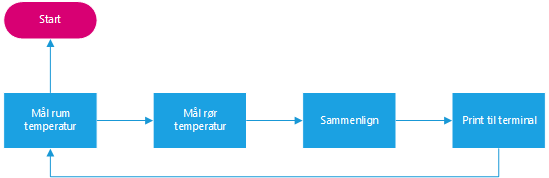
\includegraphics[width=1\textwidth]{figures/Fase1software.png}
  \caption{Fase 1 - Software flowchart.}
\end{figure}



\subsection{Mål rum temperatur}

\subsection{Mål rør temperatur}

\subsection{Sammenlign}

\subsection{Print til terminal}

\begin{figure}[h!]
  \centering
  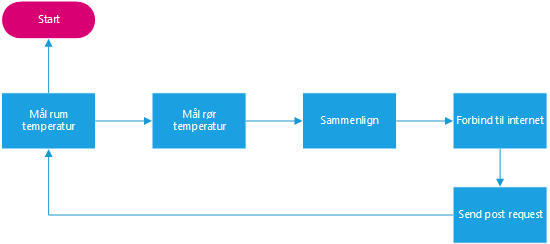
\includegraphics[width=1\textwidth]{figures/Fase2software.png}
  \caption{Fase 2 - Software flowchart.}
\end{figure}